\chapter{A trait-based characterization of phytoplankton communities in contrasting environmental regions of the Atlantic Ocean}

\small {\textbf{Manuscript to be submitted to Marine Ecology Progress Series}}

%\subsection*{}
%\textbf{ABSTRACT}: In recent years trait-based ecology studies had been providing new insights on the mechanisms driving natural variation based on measurable key characteristics of organisms. Here we investigate the phytoplankton community size-composition in the Atlantic Ocean using data from the Atlantic Meridional Transect program. We extended the existing knowledge on the distribution of the phytoplankton size composition in the Atlantic, using a larger data set, integrating phytoplankton size composition, nutrients concentrations, and grazers abundance into a trait-based approach. The selected subset was constrain by k-means partitioning and based on the prevailing environmental conditions. Also we studied how the different phytoplankton size fractions respond to different environmental gradients. Our results suggest a linkage of the \textit{in situ} environmental conditions with community size-composition, and regardless of the spatio-temporal conditions. We discuss how the observed patterns of phytoplankton size-fractions in the Atlantic Ocean are coherent with the niche partitioning theory and opposed to the unified neutral theory of biodiversity.

\normalsize
\section{Introduction}
For decades ecologists have been trying to understand how the structure of phytoplankton communities is associated to the environmental conditions, with a particular focus on the causes and consequences of natural variation. One of the approaches adopted in this important quest is based on observations of key characteristics of organisms, populations or communities. These key characteristics are also called traits \citep{McGill2006, Violle2007}. Trait-based ecology aims at developing an understanding and a better predictability of natural communities by linking traits that influence organism performance and fitness to prevailing environmental conditions \citep{McGill2006}. 

Phytoplankton communities are ideal systems for the application of a trait-based approach. They are relatively simple and have well defined ecological niches, which are determined by physical and environmental conditions, by resource allocation strategies, and by inter-specific relationships \citep{Litchman2007}. Phytoplankton organisms have various well-understood morphological, physiological, behavioural, and life history traits. Among a number of potentially relevant traits, cell size is probably the one that can best characterize phytoplankton communities, because many ecophysiological processes such as nutrient and light acquisition and resistance to grazing are significantly correlated with cell size \citep{Litchman2008,Litchman2010}. A variety of these traits are frequently measured \textit{in vivo} and \textit{in situ} due to the global importance of phytoplankton as a primary producer with a significant influence on the marine food-webs and on the biogeochemical cycles of major nutrients\citep{Falkowski1998}.

Since 1995 two scientific cruises of the Atlantic Meridional Transect (AMT) Programme have crossed the Atlantic Ocean from Plymouth (UK) to South America or South Africa almost every spring and autumn. The information collected during these cruises includes data on size-fractionated chlorophyll-a, on the concentrations of nitrate, nitrite, phosphate and silicate, on temperature, and on zooplankton abundances. The spatial extent of the transects, that cross a range of ecosystems from sub-polar to tropical and from euphotic shelf seas and upwelling systems to oligotrophic mid-ocean gyres, and the richness of the variables observed, make the dataset important for studying the size compositions of phytoplankton communities and the processes shaping them at an ocean basin scale. Previous analyses have focused on a description of the occurrences of the different size fractions \citep{Maranon2001}, but did not consider the direct influence of environmental conditions on the community structure. A more comprehensive analysis that includes the most recent observations and integrates the relevant environmental data with the available phytoplankton community size fractions is to our knowledge still lacking. The work we present here therefore intends to investigate the mechanisms determining the phytoplankton community structure in regions of contrasting environmental conditions (i.e. regions with different nutrient, temperature, and grazing regimes).

We broaden previous analyses by considering a larger and most up-to-date selection of data than any previous study. More specifically, we integrate phytoplankton size-fractions with temperature, various nutrient concentrations, and zooplankton abundances in a first attempt to disentangle the relative contribution of bottom-up and top-down processes in shaping the size structure of the phytoplankton community.

The first step in our analysis is to spatially separate the selected AMT dataset according to the well-established ecological classification of the world ocean by \citet{Longhurst2006}. In a second step, we classify the phytoplankton communities by using only the corresponding nutrients and temperature data and compare the results with the classification of \citet{Longhurst2006}. In a last step, we relate the environmental differences to the cell size compositions in order to highlight the emergent patterns of community structures at the ocean basin scale.

\section{Methods}

\begin{figure}
\centering
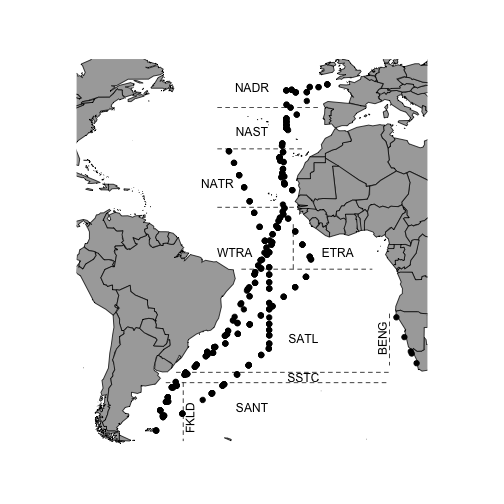
\includegraphics[trim = 30mm 20mm 25mm 20mm, clip, width=0.5\linewidth]{./Chp2-Pre/amt_mapFINAL2.png}
\caption[Scheme]{\small {The AMT subset of 410 samples used in this study. The dashed lines represent the simplified limits of the Longhurst (2006) ecological provinces.}}
\label{Map}
\end{figure}

We collected a number of observed variables from the AMT Programme (www.amt-uk.org). The resulting dataset comprised size fractionated chlorophyll-a (phytoplankton size fractions hereafter), nitrate+nitrite, phosphate and silicate concentrations, temperature, and zooplankton abundance (considered as a qualitative indication of grazing pressure). We restricted our selection to the mixed layer depth, defined as the depth at which a variation of 0.5 $^\circ$C in temperature and of 0.125 in density is observed with respect to the surface value (i.e. the value at 5-10 m depth). The resulting dataset included 410 samples from a total of 9 AMT cruises (from AMT2 to AMT6, AMT10, AMT11, AMT13, and AMT14). These cruises took place in April-May or September-October of 1996 (AMT2 and AMT3), 1997 (AMT4 and AMT5), 1998 (AMT6), 2000 (AMT10 -AMT11), and 2003 (AMT13 and AMT14). 

During most of the cruises the phytoplankton size fractions were in the range of 0.2-2 $\mu$m (picoplankton), 2 -20 $\mu$m (nanoplankton), and $>$20 $\mu$m (microplankon), although AMT13 and AMT14 measured four size classes (0.2-2, 2-5 5-10, $>$10 $\mu$m). For consistency, we considered the 2-5 and 5-10 $\mu$m size classes as part of the nanoplankton and the $>$10 $\mu$m class as part of the microplankton. The three size fractions were then normalized according to the proportion of each size fraction to the total chlorophyll-a concentration.

The selected dataset covered temperate, subtropical and tropical regions of the Atlantic Ocean (Figure \ref{Map}). Following Longhurst's (\citeyear{Longhurst2006}) classification, ten ecological provinces were sampled by the AMT cruises: four temperate provinces, comprising of the North Atlantic Drift (NADR; 24 samples), the South Subtropical Convergence (SSTC, n=21), the Subantartic Water Ring (SANT, n=14), and the Falkland Island (FKLD; 52 samples); two subtropical provinces, comprising of the North Atlantic Subtropical Gyral (NAST; 37 samples) and the South Atlantic Subtropical Gyral (SATL, 129 samples); three tropical provinces, the North Atlantic Tropical Gyral (NATR, 51 samples), the Eastern Tropical Atlantic (ETRA, 13 samples) and the Western Tropical Atlantic (WTRA, 64 samples); and one upwelling region, the Benguela province (BENG, 5 samples). With this dataset the phytoplankton community size composition was analyzed by means of a linear mixed effect model (LME) to test if the community size-structure differs among ecological provinces. The ecological provinces were classified into regions, defined as: temperate (NADR, FKLD, SSTC, SANT), tropical (NATR, WTRA, ETRA), subtropical (SATL, NAST) and upwelling (BENG). The model was fitted to the data using the size fractions and the regions as fixed factors, and the ecological provinces as randomly varying factors.

We utilized a cluster analysis based on the $k$-means algorithm (a statistical method that partitions $n$ observations into $k$ clusters in which each observation belongs to the cluster with the nearest mean) to alternatively classify the data with respect to the prevailing environmental conditions. The environmental variables considered were nitrate+nitrite, phosphate and silicate concentrations, and temperature. 

We also applied a principal component analysis (PCA) to the environmental variables and the normalized size fractions to assess the effect of a specific environmental gradient to changes in the phytoplankton size fractions. We quantified the linear relationships between the environmental data and the size-structure information. 

In addition, we quantified the relation of the three size fractions to the grazer abundance relatively to AMT3 and AMT5, because zooplankton data were only available for these two cruises. These analyses were carried out using R v2.12.2 (The R Foundation for Statistical Computing, 2011).

\section{Results}

\begin{figure}
\centering
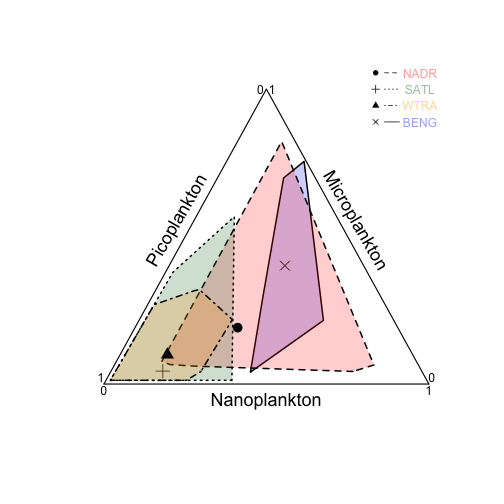
\includegraphics[trim = 20mm 30mm 20mm 20mm, clip, width=0.6\linewidth]{./Chp2-Pre/amt_4RegionsTriSizeFrac4.png}
\caption[Scheme]{\small {Phytoplankton community size structure of four ecological provinces in the Atlantic Ocean. The contours correspond to the convex hull of the size-fraction distribution of each province. The symbols indicate the corresponding mean values.}}
\label{RegSizeFrac}
\end{figure}

\begin{figure}
\centering
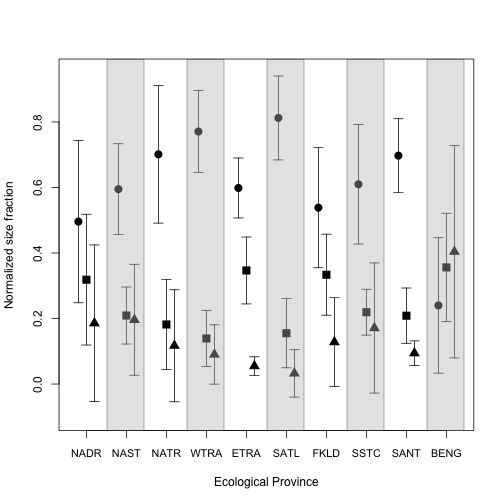
\includegraphics[trim = 0mm 0mm 0mm 0mm, clip, width=0.9\linewidth]{./Chp2-Pre/amt_MeanSDProvinces.png}
\caption[Scheme]{\small {Relative mean abundances ($\pm$sd) of three phytoplankton size fractions of ten ecological provinces of the Atlantic Ocean. The symbols indicate the mean values of the normalized size fractions: picoplankton (\ding{108}), nanoplankton(\ding{110}) and microplankton (\ding{115}).}}
\label{means}
\end{figure}

The size-structure of the phytoplankton communities is highly variable in different ecological provinces of the Atlantic Ocean (Figure \ref{RegSizeFrac}). When the mean size-fraction of only four selected provinces are compared, an increasing trend towards bigger phytoplankton sizes can be observed from the warmer provinces of the tropics and subtropics to the colder provinces of, for example, the Benguela upwelling. In tropical and subtropical waters (such as WTRA and SATL), picoplankton is the most common size class, with only a few occurrences of nano- and microplankton. In contrast, temperate provinces such as NADR are characterised by a more heterogeneous distribution of size classes and the upwelling province is dominated mainly by pico- and microplankton. Provinces located in the temperate regions have a larger cell size variability, as indicated by the larger standard deviation there than in the provinces located in the tropical regions (Figure \ref{means}). These differences are rather significant for the picoplankton (LME/anova, df=3, F=6.6315, p=0.0247) and the microplankton (LME/anova, df=3, F=5.5189,p=0.0368) size fractions, while they are less significant for the nanoplankton (LME/anova, df=3, F=2.03341, p=0.2108) size fractions.

\begin{figure}
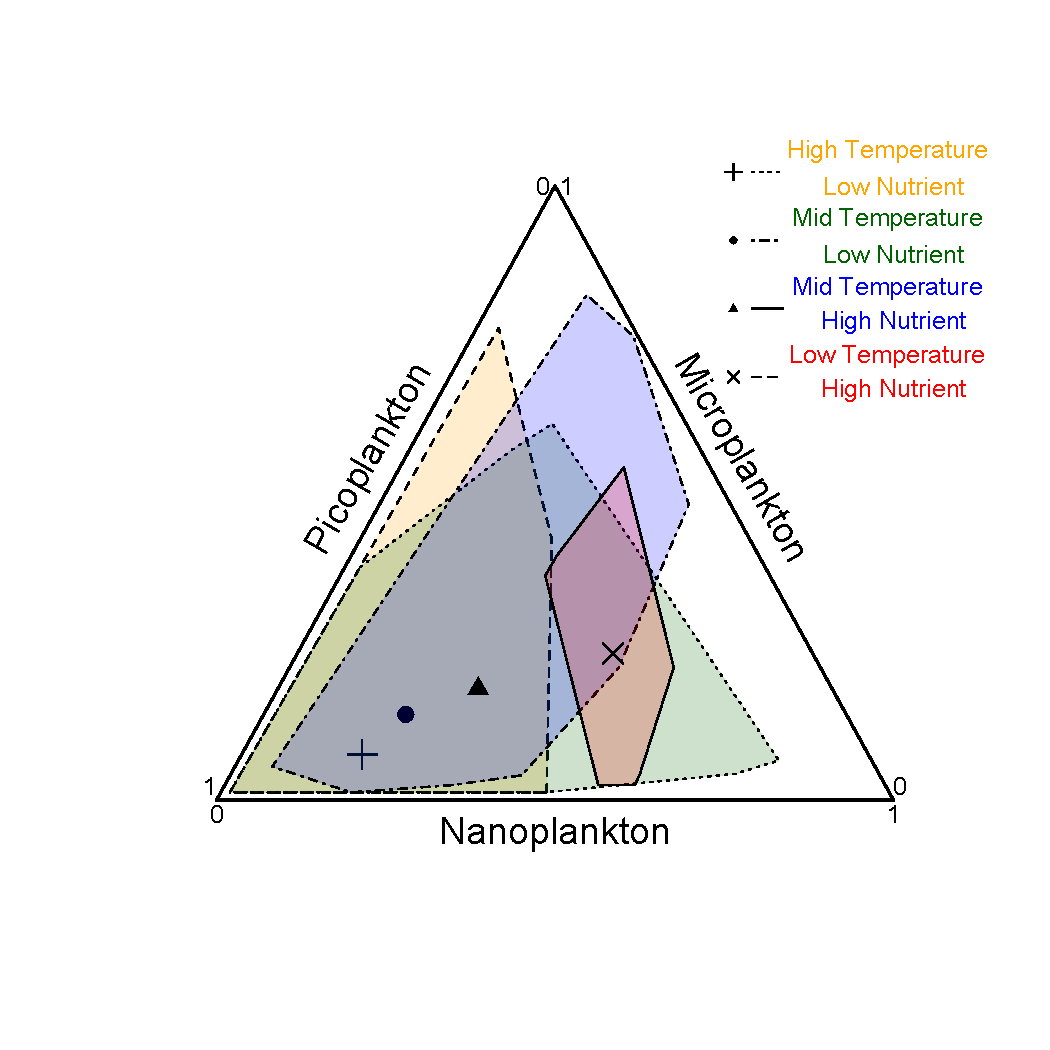
\includegraphics[trim = 12mm 15mm 10mm 15mm, clip, width=0.5\linewidth]{./Chp2-Pre/amt_clsEnvFINAL4-5.pdf}
\put(1,210){\textbf{b)}}
\put(-180,210){\textbf{a)}}
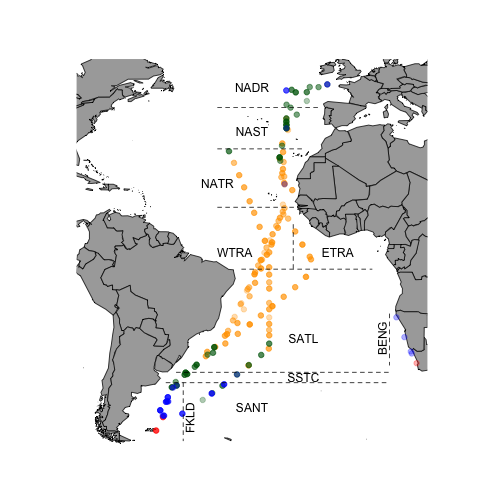
\includegraphics[trim = 20mm 20mm 20mm 20mm, clip, width=0.5\linewidth]{./Chp2-Pre/amt_mapClsEnv3.png}
\caption[Scheme]{\small {Phytoplankton community size structure and environmental conditions. a) Distributions of size-classes clustered according to water temperature and nutrient concentration with contours corresponding to the convex hull of the size-fraction distribution of each cluster; symbols denoting the mean values of the size fractions. b) Geographical distribution of the clusters compared to Longhurst provinces. The colour coding reflects the cluster classification.}}
\label{clusters}
\end{figure}

\begin{table}
\centering
\caption[Scheme]{\small {Mean values of environmental parameters for the different clusters: High temperature - Low nutrients (HTLN), Mid temperature - Low nutrients (MTLN), Mid temperature - High nutrients (MTHN and Low temperature - High nutrients (LTHN).}}
\label{tableclus}
\begin{tabular} {c c c c c}
cluster & NO$_2^-$ + NO$_3^-$ & PO$_4^{3-}$ & SiO$_4^{2-}$ & Temperature \\ \hline
HTLN & 0.150$\pm$0.575 & 0.064$\pm$0.078 & 1.097$\pm$0.575 & 25.299$\pm$2.000 \\
MTLN & 0.556$\pm$1.102 & 0.112$\pm$0.141 & 0.816$\pm$0.617 & 17.894$\pm$2.191 \\
MTHN & 9.027$\pm$3.593 & 0.799$\pm$0.373 & 2.423$\pm$1.375 & 11.925$\pm$2.797 \\
LTHN & 30.324$\pm$4.549 & 1.336$\pm$0.208 & 4.590$\pm$1.926 & 6.810$\pm$3.435 \\ \hline
\end{tabular}
\end{table}

The $k$-means clustering analyses of temperature, nitrate+nitrite, phosphate, and silicate concentrations reveals that regions between 30$^{\circ}$ North and South share similar environmental characteristics of high temperatures and low nutrient concentrations (HTLN, yellow dots in Figure \ref{clusters}b, cf. Table \ref{tableclus}). Observations from temperate provinces are clearly separated from HTLN data. They are categorized into three clusters: Mid temperature - Low nutrients, Mid temperature - High nutrients and Low temperature - High nutrients (respectively green, blue and red dots in Figure \ref{clusters}b, cf. Table \ref{tableclus} ). In summary, we obtained a new classification of the data into four regions, which explains 87.3\% of the variance. The mean size of phytoplankton in the four clusters indicates an increasing trend from the high-temperature, low-nutrient region towards the low-temperature, high-nutrient regions (Figure \ref{clusters}a). The PCA on all data shows highest loadings for temperature (positive loading) and nitrate+nitrite concentration (negative loading) with respect to the first principal component (Figure \ref{PrinComp}). Furthermore, the relative occurrence of picoplankton is positively correlated with temperature, while nutrient concentrations are positively correlated with occurrences of nano- and microplankton (Figure \ref{PrinComp}).

The results of the regression analyses of all data show that phytoplankton size composition varies with the environmental conditions irrespective of temporal changes (see Figure \ref{response1} and Table \ref{stats}). A shift from a picoplankton dominated community towards a nano- and microplankton dominated community occurs with increasing nutrient concentrations (see Figure \ref{response1}a, \ref{response1}b and \ref{response1}c). By contrast, the relative abundance of picoplankton increases from about 40\% to about 80\% with a temperature increase from 4.8-9$^{\circ}$C to 25-29$^{\circ}$C, whereas the fractions of nano- and microplankton decreases by about 50\%.

When restricting the regression analysis to the only two cruises that also sampled zooplankton (AMT3 and AMT5), we observe an increase in copepod abundance in association to a decline in the relative occurrence of picoplankton from 70$\%$ to less than 40$\%$ and an increase of the relative occurrence of nanoplankton from 20$\%$ to 60$\%$. The microplankton size fraction is, however, not affected by changes in the zooplankton abundance (Figure \ref{response2}).

\begin{figure}
\centering
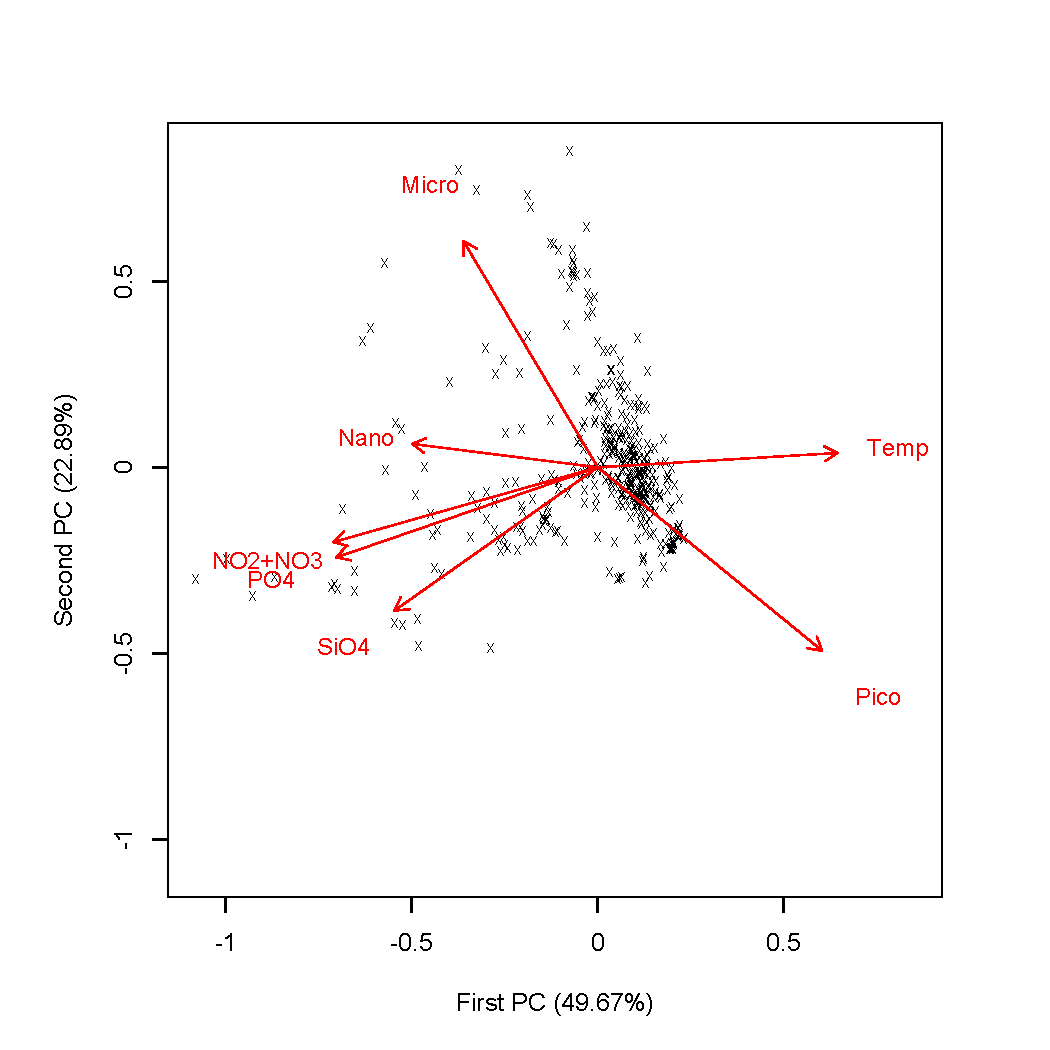
\includegraphics[trim = 0mm 0mm 0mm 0mm, clip, width=0.9\linewidth]{./Chp2-Pre/amt_PrinComp.pdf}
\caption[Scheme]{\small {Principal Component Analysis of environmental parameters and normalized phytoplankton size fractions.}}
\label{PrinComp}
\end{figure}

\begin{figure}
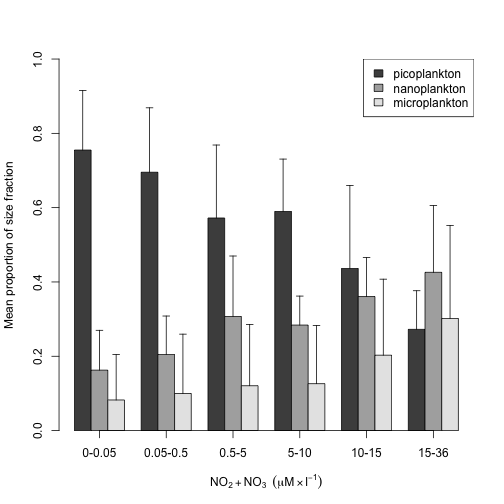
\includegraphics[trim = 0mm 0mm 0mm 15mm, clip, width=0.5\linewidth]{./Chp2-Pre/amt_NO3_bars2.png}
\put(-180,210){\textbf{a)}}
\put(1,210){\textbf{b)}}
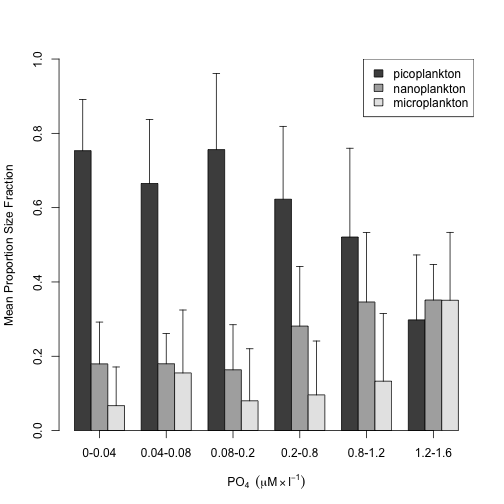
\includegraphics[trim = 0mm 0mm 0mm 15mm, clip, width=0.5\linewidth]{./Chp2-Pre/amt_PO4_bars2.png}
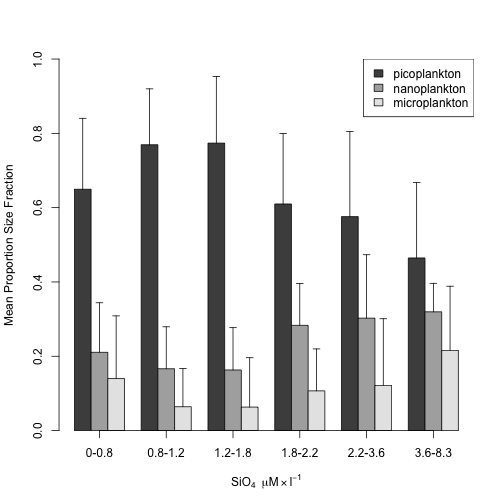
\includegraphics[trim = 0mm 0mm 0mm 15mm, clip, width=0.5\linewidth]{./Chp2-Pre/amt_SiO4_bars2.png}
\put(-180,210){\textbf{c)}}
\put(1,210){\textbf{d)}}
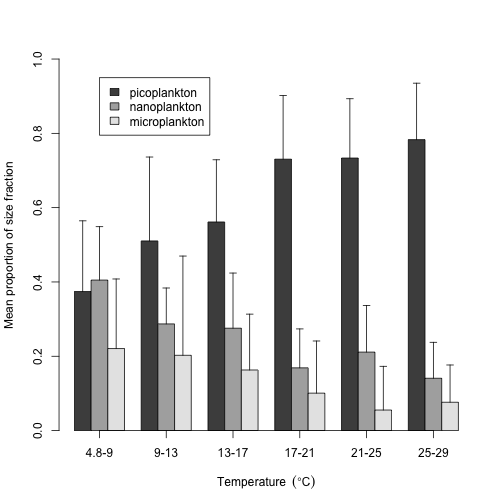
\includegraphics[trim = 0mm 0mm 0mm 15mm, clip, width=0.5\linewidth]{./Chp2-Pre/amt_Temp_bars2.png}
\caption[Scheme]{\small {Relative composition of picoplankton, nanoplankton and microplankton size fractions changing with concentrations of nitrate+nitrite (a), phosphate (b), and silicate (c) and with temperature (d). The bars represent mean values and the error bars indicate the standard deviation.}}
\label{response1}
\end{figure}

\begin{figure}
\centering
\includegraphics[trim = 0mm 0mm 0mm 15mm, clip, width=0.6\linewidth]{./Chp2-Pre/amt_zoo_bars2.png}
\caption[Scheme]{\small {Relative composition of picoplankton, nanoplankton and microplankton size fractions changing with copepod abundance. The bars represent mean values and the error bars indicate the standard deviation.}}
\label{response2}
\end{figure}

\begin{table}
\centering
\caption[Scheme]{\small {Summary statistics for linear fittings of the three size fractions to each environmental variable.}}
\label{stats}
\begin{tabular} {c c c c c c c c c c }
& \multicolumn{3} {c} {Picoplankton} & \multicolumn{3} {c} {Nanoplankton} & \multicolumn{3} {c} {Microplankton} \\
& slope & p-value & $r^2$ & slope & p-value & $r^2$ & slope & p-value & $r^2$ \\ \hline
NO$_2^-$ + NO$_3^-$ &-0.090 &0.002 & 0.908 &0.050 &0.001 & 0.921 &0.040 &0.010 &0.792 \\
PO$_4^{3-}$ &-0.0812 &0.021 &0.711 &0.042 &0.012 &0.777 &0.039 &0.125 &0.354 \\
SiO$_4^{2-}$ &-0.047 &0.085 &0.455 &0.030 &0.044 &0.597 &0.016 &0.247 &0.142 \\ 
Temperature &0.082 &0.001 &0.914 &-0.047 &0.008 &0.812 &-0.035 &0.003 &0.885 \\
Copepods &-0.063 &0.064 &0.520 &0.068 &0.051 &0.567 &-0.004 &0.788 &-0.222\\ \hline
\end{tabular}
\end{table}


\section{Discussion}
We analyzed cruise data from different regions of the Atlantic Ocean covering mainly two seasons (late spring/early summer and autumn) in the period 1996 to 2003. Our results showed, consistently with the geographical classification of \citet{Longhurst2006} (Figures \ref{RegSizeFrac} and \ref{means}), patterns of phytoplankton size distributions characterized by the dominance of picoplankton in oligotrophic (SATL) and tropical (e.g. WTRA) waters and by the dominance of larger size classes in nutrient-rich waters (BENG). These patterns are also consistent with the works of \citet{Maranon2000, Maranon2001, Poulton2006, Moreno-Ostos2011, Huete-Ortega2011}. Our new classification method, based on the prevailing environmental conditions (Figure \ref{clusters}) and independent from spatial and temporal information, maximizes differences of the environmental properties among clusters of data and generates patterns of phytoplankton size distributions similar to the ones obtained by the Longhurst's classification, which uses a richer and spatially informed dataset. The value of our approach is therefore in the fact that it leads to results consistent with the present day understanding of phytoplankton biogeography and ecology of the Atlantic without requiring information on the geographical and temporal origin of the data. Our finding also proves the generality and robustness of the trait-based approach and confirms the sensitivity of phytoplankton cell size to environmental conditions and possibly (because of the paucity of zooplankton data) to grazing pressure. In fact, the phytoplankton size compositions resulted to be strongly associated with prevailing environmental conditions (Figures \ref{response1} and \ref{response2}). Furthermore, the consistency of our results with similar previous studies of the Atlantic Ocean that used either less AMT data than our study \citep{Maranon2000, Maranon2001, Poulton2006} or data from sources different than the AMT cruises \citep{Moreno-Ostos2011, Huete-Ortega2011} suggests that the different phytoplankton size structures observed are robust features of the Atlantic Ocean.

The results we obtained with the clustering technique (Figure \ref{clusters}) revealed that the areas between 30$^\circ$ N and 30$^\circ$ S are characterized by nutrient and temperature regimes that give picoplankton a competitive advantage over larger phytoplankton. In contrast, a wider range of phytoplankton size classes distinguishes colder waters with high nutrient concentrations.

Smaller phytoplankton cell sizes have a competitive advantage over larger phytoplankton under low nutrient, low light and low grazing pressure \citep{Litchman2008, Litchman2010}. From our regression analyses (Figures \ref{response1} and \ref{response2}) we inferred a strong control of NO$_3^-$+NO$_2^-$ and temperature on all three size fractions. Pico- and nanoplankton size fractions, however, appeared more sensitive to changes in PO$_4^{3-}$, SiO$_4^{2-}$ and copepod abundance. We propose that these effects are caused by a trade-off between resource acquisition and predation pressure, although with the caveat represented by the paucity of the zooplankton data and by the qualitative value we attribute to zooplankton abundance as an indication of grazing pressure. There are a number of important physiological and ecological processes that strongly depend on phytoplankton cell size \citep{Kiorboe1993, Cermeno2008a, Finkel2009a}, including metabolic rates, maximum nutrient uptake rate, nutrient diffusion, light absorption, sinking velocity, trophic interactions and even diversity within taxa, which is often a log-normal distribution of body size. Our results are therefore consistent with this general "size rule" \citep{Finkel2009a}. To our knowledge it is the first time that this feature is observed in data extending across an entire ocean basin and irrespective of temporal changes.

Our size-based analyses therefore substantiate remarkable properties of the variation of a key trait at an ocean basin scale. Moreover, these findings are corroborating Baas Becking's tenet "everything is everywhere, but the environment selects" \citep{BaasBecking1934} over a large-scale environmental gradient. Here we evidenced how the partitioning of resources along our selected trait, phytoplankton size, is a strong feature at an ocean basin scale. These observations lend weight to arguments supporting the niche partitioning theory rather than the unified neutral theory of biodiversity. The importance of the finding that the prevailing environmental condition is the major driver of the phytoplankton community structure in the Atlantic Ocean need to be further investigated using the trait-based modelling approach of \citet{Bruggeman2007, Merico2009}. This modelling tool will help to disentangle the relative contributions of the top-down vs. bottom-up processes in shaping the phytoplankton community structure, a research direction also promoted very recently by \citet{Follows2011}.

\section{Acknowledgements}
This study uses data from the Atlantic Meridional Transect Consortium (NER/0\\/5/2001/00680), provided by the British Oceanographic Data Centre and supported by the Natural Environment Research Council. 
